% ============================================================================
%  Modernizing DeepSORT: Selectable Detectors, Re-Identification Models, and a
%  Standalone Body-REID Identity System for Multi-Object Tracking
%  ---
%  HSE Final Project Report. LaTeX source (Overleaf / pdflatex compatible).
% ============================================================================

\documentclass[12pt, a4paper]{article}

% Encoding and language
\usepackage[utf8]{inputenc}
\usepackage[T1]{fontenc}
\usepackage[english]{babel}

% Typography
\usepackage{mathptmx}
\usepackage{microtype}
\usepackage{setspace}
\onehalfspacing

% Page geometry
\usepackage[left=30mm, right=15mm, top=20mm, bottom=20mm]{geometry}

% Mathematics
\usepackage{amsmath, amssymb}

% Graphics and figures
\usepackage{graphicx}
\usepackage{float}
\usepackage{subcaption}
\graphicspath{{images/outputs/}}
\usepackage[section]{placeins}

% Tables
\usepackage{booktabs}
\usepackage{array}
\usepackage{multirow}
\usepackage{tabularx}

% Code listings
\usepackage{listings}
\usepackage{xcolor}
\definecolor{codebg}{HTML}{F7F7F8}
\definecolor{codegreen}{HTML}{2E7D32}
\definecolor{codegray}{HTML}{6B7280}
\definecolor{codepurple}{HTML}{7C3AED}
\lstdefinestyle{pythonstyle}{
  backgroundcolor=\color{codebg}, basicstyle=\ttfamily\footnotesize,
  keywordstyle=\color{codepurple}\bfseries, commentstyle=\color{codegray}\itshape,
  stringstyle=\color{codegreen}, breaklines=true, frame=single,
  rulecolor=\color{codebg}, numbers=left, numberstyle=\tiny\color{codegray},
  tabsize=4, showstringspaces=false, language=Python,
}
\lstset{style=pythonstyle}

% Hyperlinks
\usepackage[colorlinks=true, linkcolor=blue!60!black, citecolor=blue!60!black,
  urlcolor=blue!60!black]{hyperref}

% Bibliography
\usepackage[numbers, sort&compress]{natbib}

% Captions
\usepackage[font=small, labelfont=bf]{caption}

% Custom commands
\newcommand{\hota}{\textsc{hota}}
\newcommand{\osnet}{\textsc{OSNet}}
\newcommand{\reid}{\textsc{reid}}

\setcounter{secnumdepth}{3}
\setcounter{tocdepth}{3}

% ============================================================================
\begin{document}

% ----------------------------------------------------------------------------
%  TITLE PAGE
% ----------------------------------------------------------------------------
\begin{titlepage}
\begin{center}

\textbf{Federal State Autonomous Educational Institution \\
of Higher Education} \\[4pt]
\textbf{``National Research University ``Higher School of Economics''} \\[24pt]

\rule{\textwidth}{0.4pt} \\[12pt]

{\large Faculty of Informatics, Mathematics, and Computer Science} \\[6pt]
{\large Master's Programme ``Artificial Intelligence and Computer Vision''} \\[6pt]
{\large Master of Science} \\[24pt]

\vspace{1cm}

{\LARGE \bfseries REPORT} \\[6pt]
{\large on the Final Project} \\[18pt]

\rule{0.8\textwidth}{0.4pt} \\[12pt]

{\Large \bfseries
Modernizing DeepSORT: Selectable Detectors, \\
Re-Identification Models, and a Standalone \\
Body-REID Identity System for Multi-Object Tracking
} \\[24pt]

\rule{0.8\textwidth}{0.4pt}

\vfill

\begin{flushleft}
\begin{tabular}{p{0.5\textwidth} p{0.4\textwidth}}
\textbf{Completed by:} & \\
Student Sergei Solovev & \rule{4cm}{0.4pt} \\
 & {\small (signature)} \\[18pt]
\textbf{Reviewed by:} & \\
Course instructor & \rule{4cm}{0.4pt} \\
 & {\small (signature and date)} \\
\end{tabular}
\end{flushleft}

\vspace{1cm}
{\large Moscow, 2026}

\end{center}
\end{titlepage}

\newpage
\tableofcontents
\newpage

% ----------------------------------------------------------------------------
%  ABSTRACT
% ----------------------------------------------------------------------------
\section*{Abstract}
\addcontentsline{toc}{section}{Abstract}

This report describes the modernization of the DeepSORT multi-object tracker. The original
DeepSORT consumes precomputed detections and a fixed appearance encoder; this work replaces those
fixed components with selectable modern object detectors and re-identification (\reid{}) models while
keeping the Kalman-filter and Hungarian-assignment core unchanged. The detector and \reid{} backends
are wired behind two adapter interfaces with a lazy-import registry, so models from different source
libraries can be selected before a run without touching the tracking core. A segmentation detector
and a standalone body-\reid{} identity component are added as optional modules.

The system is evaluated on six MOT-Challenge sequences (TUD-Campus, TUD-Stadtmitte, KITTI-17 and
PETS09-S2L1 from the 2D~MOT~2015 benchmark; MOT16-09 and MOT16-11 from MOT16) using the
Higher-Order Tracking Accuracy (\hota{}) metric computed with TrackEval. The unmodified baseline
reaches a mean \hota{} of $40.17$. The best modern configuration (YOLOv8m detector with an \osnet{}
\reid{} model) reaches a mean \hota{} of $52.54$ ($+12.37$ absolute), exceeds the baseline on each of
the six videos, and runs at $9.87$ frames per second on a single Tesla~T4 (above the $5$~FPS
real-time threshold). A per-video tuning study on TUD-Campus and an analysis of the
environment-related build failures encountered during the project are reported, including the cases
that did not work as expected.

\textbf{Keywords:} multi-object tracking, DeepSORT, person re-identification, HOTA, MOT-Challenge,
YOLOv8, OSNet, segmentation.

\newpage

% ----------------------------------------------------------------------------
%  1. GENERAL DESCRIPTION
% ----------------------------------------------------------------------------
\section{General Description of the Project}
\label{sec:general}

\subsection{Project Type}
This is an applied engineering and research project. It involves re-engineering an existing
open-source tracker into a configurable system, integrating several third-party detection and
re-identification models, running controlled experiments on a public benchmark, and reporting both
quantitative results and the failures encountered during development.

\subsection{Context and Motivation}
Multi-object tracking (MOT) assigns a consistent identity to each detected object across the frames
of a video. DeepSORT~\cite{wojke2017deepsort} extends SORT~\cite{bewley2016sort} by adding an
appearance descriptor to the motion-based association of the original tracker. The reference
implementation, however, predates current detection and re-identification models: it reads
precomputed detections from disk and uses a single fixed appearance encoder
(\texttt{mars-small128})~\cite{wojke2018cosine}. The goal of this project is to modernize the tracker
so that current detectors and re-identification models can be selected at run time, and to measure
whether the modernized tracker improves tracking accuracy over the original baseline while remaining
real-time.

\subsection{Problem Statement}
Given a sequence of frames, the tracker must output, for every frame, a set of bounding boxes each
labelled with a persistent track identity. The integration contract of the original tracker is kept:
each detection is represented as a \texttt{Detection(tlwh, confidence, feature)} object and passed to
\texttt{tracker.predict()} followed by \texttt{tracker.update()}. The objective is to maximize the
mean \hota{} across the six evaluation videos, subject to a real-time constraint of at least
$5$~FPS for at least one configuration, while keeping the SORT core unchanged.

\subsection{Dataset}
\label{sec:dataset}
All six evaluation sequences are taken from the training splits of the MOT-Challenge benchmarks, so
ground-truth annotations are available for scoring. Four sequences come from 2D~MOT~2015
\cite{leal2015motchallenge} and two from MOT16~\cite{milan2016mot16}. Table~\ref{tab:dataset}
summarizes them.

\begin{table}[H]
\centering
\caption{Evaluation sequences. Frame counts are the standard MOT-Challenge values.}
\label{tab:dataset}
\begin{tabular}{llcc}
\toprule
\textbf{Sequence} & \textbf{Benchmark} & \textbf{Frames} & \textbf{Scene} \\
\midrule
TUD-Campus     & 2D MOT 2015 & 71  & outdoor, crossing pedestrians \\
TUD-Stadtmitte & 2D MOT 2015 & 179 & outdoor, street \\
KITTI-17       & 2D MOT 2015 & 145 & street, moving camera \\
PETS09-S2L1    & 2D MOT 2015 & 795 & outdoor, surveillance \\
MOT16-09       & MOT16       & 525 & indoor, pedestrians \\
MOT16-11       & MOT16       & 900 & indoor, pedestrians \\
\bottomrule
\end{tabular}
\end{table}

A 10-column versus 9-column difference in the ground-truth format of the two benchmarks is discussed
in Section~\ref{sec:difficulties}; it affected an early version of the data loader.

\subsection{Evaluation Protocol and Metrics}
\label{sec:protocol}
The primary metric is \hota{}~\cite{luiten2021hota}, which combines a detection accuracy term
(DetA) and an association accuracy term (AssA) into a single value and is computed with
TrackEval~\cite{trackeval}. MOTA, IDF1, DetA and AssA are reported as secondary metrics. Three
screening procedures are used in addition to end-to-end \hota{}:
\begin{itemize}
  \item detector quality is scored independently as precision, recall and F1 against ground truth at
        an intersection-over-union threshold of $0.5$;
  \item the re-identification model is screened by running the tracker on ground-truth boxes (the
        detector is replaced by ground truth), so that \hota{} differences reflect appearance only;
  \item the standalone body-\reid{} component is screened as a clustering problem on ground-truth
        crops using the Fowlkes-Mallows index, the silhouette coefficient and the
        Calinski-Harabasz index.
\end{itemize}
Speed is measured by \texttt{eval/fps\_bench.py} with the detector, \reid{} and tracker stages timed
separately after a warm-up. Every run appends a row to \texttt{results/experiments.csv} so that the
experimental history is reproducible.

% ----------------------------------------------------------------------------
%  2. BACKGROUND
% ----------------------------------------------------------------------------
\section{Background and Related Work}
\label{sec:background}

\subsection{SORT and DeepSORT}
SORT~\cite{bewley2016sort} performs tracking-by-detection using a Kalman filter for motion prediction
and the Hungarian algorithm for frame-to-frame assignment based on bounding-box overlap. DeepSORT
\cite{wojke2017deepsort} adds an appearance descriptor and a cosine distance gate, which reduces
identity switches through occlusions. The appearance encoder of the reference implementation is the
\texttt{mars-small128} cosine-metric-learning network~\cite{wojke2018cosine}.

\subsection{Modern Detectors}
Three detector families from three source repositories were integrated: YOLOv8 from
Ultralytics~\cite{jocher2023yolov8}, NanoDet~\cite{rangilyu2021nanodet}, and RTMDet from
MMDetection~\cite{lyu2022rtmdet, mmdetection}. A YOLOv8 segmentation variant is also integrated and
converts the predicted mask to a bounding box.

\subsection{Re-Identification Models}
Re-identification models map a cropped person image to an embedding such that crops of the same
person are close under cosine distance. \osnet{}~\cite{zhou2019osnet} is a compact
re-identification network; it is used here through the BoxMOT package~\cite{brostrom2023boxmot},
which bundles weights trained on MSMT17. A generic ImageNet backbone from
\texttt{timm}~\cite{wightman2019timm} is used as a dependency-light fallback. The torchreid
library~\cite{zhou2021torchreid} provides additional \osnet{} variants.

\subsection{The HOTA Metric}
\hota{}~\cite{luiten2021hota} was proposed to balance detection and association in a single score,
addressing known biases of MOTA (detection-dominated) and IDF1. It is the metric used by recent
MOT-Challenge evaluations and is the primary target of this project.

% ----------------------------------------------------------------------------
%  3. EXECUTION PROCESS
% ----------------------------------------------------------------------------
\section{Description of the Project Task Execution Process}
\label{sec:process}

\subsection{Architecture and Integration Contract}
The tracking core (\texttt{deep\_sort/}: Kalman filter, track, tracker, linear assignment, IoU
matching, detection) is kept unchanged except for one guard in the nearest-neighbour metric that
makes the appearance distance dimension-agnostic, so that embeddings of different sizes
($128$, $512$, $\sim1280$, $2048$) can be used without further changes. Detection and
re-identification are placed behind two abstract interfaces, \texttt{BaseDetector} and
\texttt{BaseReIDExtractor}, each resolved by a lazy-import registry so that a backend that fails to
install does not block the others. Figure~\ref{fig:pipeline} shows the data flow.

\begin{figure}[H]
  \centering
  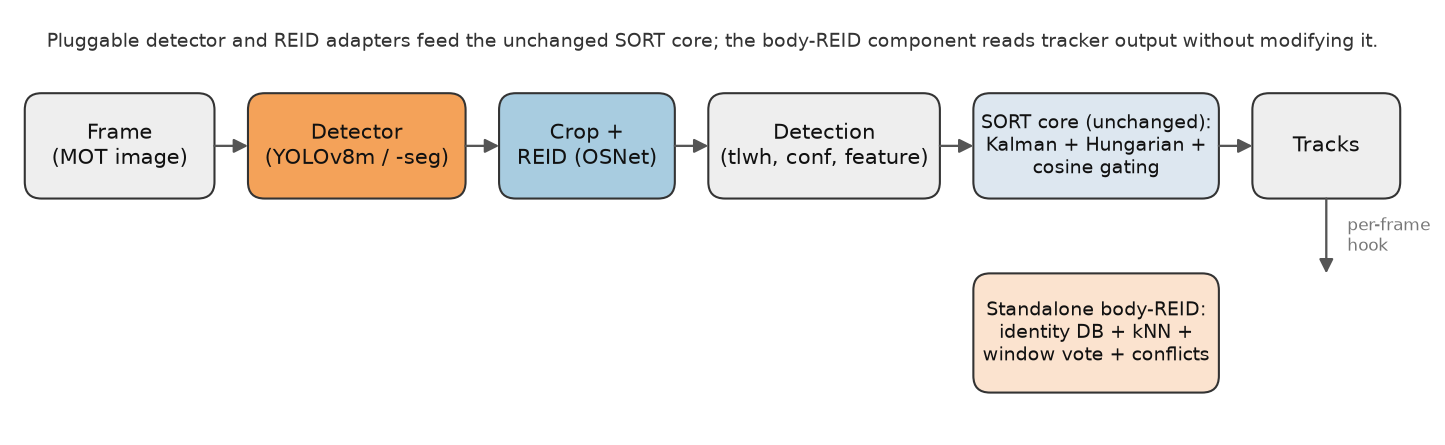
\includegraphics[width=0.95\textwidth]{fig_pipeline.png}
  \caption{Data flow. Pluggable detector and \reid{} adapters feed the unchanged SORT core; the
  standalone body-\reid{} component reads tracker output through a per-frame hook without modifying
  the core.}
  \label{fig:pipeline}
\end{figure}

\subsection{Stage 0: Environment}
The development environment is a Windows workstation for authoring and Google Colab Pro (Tesla T4,
Python~3.12) for all compute. The notebook \texttt{notebooks/DeepSORT\_Modern.ipynb} is a thin
orchestrator: it clones the repository and calls the scripts in \texttt{eval/}, \texttt{data/} and
\texttt{bodyreid/}, so that the logic lives in version-controlled modules rather than in notebook
cells.

\subsection{Stage 1: Data Preparation}
\texttt{data/download\_mot.py} downloads 2D~MOT~2015 and MOT16 and lays them out in the directory
structure expected by TrackEval. \texttt{data/prepare\_gt\_crops.py} exports ground-truth person
crops labelled by track identity for the standalone body-\reid{} study; it produced $21{,}105$ crops
over the six sequences.

\subsection{Stage 2: Baseline Reproduction}
\texttt{eval/run\_baseline.py} reproduces the unmodified DeepSORT through the original
\texttt{deep\_sort\_app.run} entry point using the provided detections and the
\texttt{mars-small128} encoder with the original tracker settings. Its output is scored under the
tracker name \texttt{baseline}.

\subsection{Stage 3: Detector Study}
\texttt{eval/det\_eval.py} runs each detector over every sequence and reports precision, recall and
F1 against ground truth at IoU~$\geq 0.5$.

\subsection{Stage 4: Re-Identification Study}
\texttt{eval/reid\_eval.py} runs the tracker on ground-truth boxes and varies only the
re-identification model, so the resulting \hota{} reflects appearance association in isolation.

\subsection{Stage 5: Full Pipeline and Per-Video Tuning}
\texttt{eval/run\_tracking.py} runs the complete live pipeline and writes MOT-format results that are
scored by \texttt{eval/trackeval\_runner.py}. Per-video parameters are set through sequence presets
in \texttt{configs/sequences/}, which are merged automatically. The TUD-Campus preset was tuned with
\texttt{eval/tune\_tud\_campus.py} (Section~\ref{sec:tuning}).

\subsection{Stage 6: Standalone Body-REID and Segmentation}
The standalone body-\reid{} identity component (Section~\ref{sec:bodyreid-method}) and the YOLOv8
segmentation detector were added as optional modules and evaluated separately.

% ----------------------------------------------------------------------------
%  4. RESULTS
% ----------------------------------------------------------------------------
\section{Description of the Project Results}
\label{sec:results}

All numbers in this section are from the live Colab runs recorded in
\texttt{results/experiments.csv} and \texttt{report/results\_table.md}. The headline tracking,
re-identification and body-\reid{} results are from the run of 2026-06-19; the detector and
segmentation studies were refreshed on 2026-06-25 with the then-current YOLOv8m weights.

\subsection{Baseline}
Table~\ref{tab:baseline} reports the per-video \hota{} of the unmodified DeepSORT. Its mean of
$40.17$ is the threshold that every modern configuration must exceed.

\begin{table}[H]
\centering
\caption{Per-video \hota{} of the unmodified DeepSORT baseline.}
\label{tab:baseline}
\small
\setlength{\tabcolsep}{4.5pt}
\begin{tabular}{lccccccc}
\toprule
 & TUD-Campus & TUD-Stadt. & KITTI-17 & PETS09 & MOT16-09 & MOT16-11 & \textbf{Mean} \\
\midrule
HOTA & 39.86 & 36.75 & 43.41 & 44.84 & 36.24 & 39.95 & \textbf{40.17} \\
\bottomrule
\end{tabular}
\end{table}

\subsection{Detector Evaluation}
Figure~\ref{fig:detprf} and Table~\ref{tab:detector} report detector precision, recall and F1.
YOLOv8m has high mean recall ($0.828$) but its precision varies by sequence: it is high on the
cleaner videos and lowest on the dense low-resolution KITTI-17 clip (precision $0.51$), where it
produces many false-positive boxes. NanoDet and RTMDet were not installed on the
runtime (Section~\ref{sec:difficulties}).

\begin{table}[H]
\centering
\caption{Detector evaluation against ground truth (mean over six videos, IoU~$\geq 0.5$).}
\label{tab:detector}
\begin{tabular}{lccc}
\toprule
\textbf{Detector} & \textbf{Precision} & \textbf{Recall} & \textbf{F1} \\
\midrule
YOLOv8m (box)            & 0.721 & 0.828 & 0.765 \\
YOLOv8m-seg (mask-to-box) & 0.727 & 0.827 & 0.768 \\
NanoDet                  & \multicolumn{3}{c}{not installed on this runtime} \\
RTMDet (MMDetection)     & \multicolumn{3}{c}{not installed on this runtime} \\
\bottomrule
\end{tabular}
\end{table}

\begin{figure}[H]
  \centering
  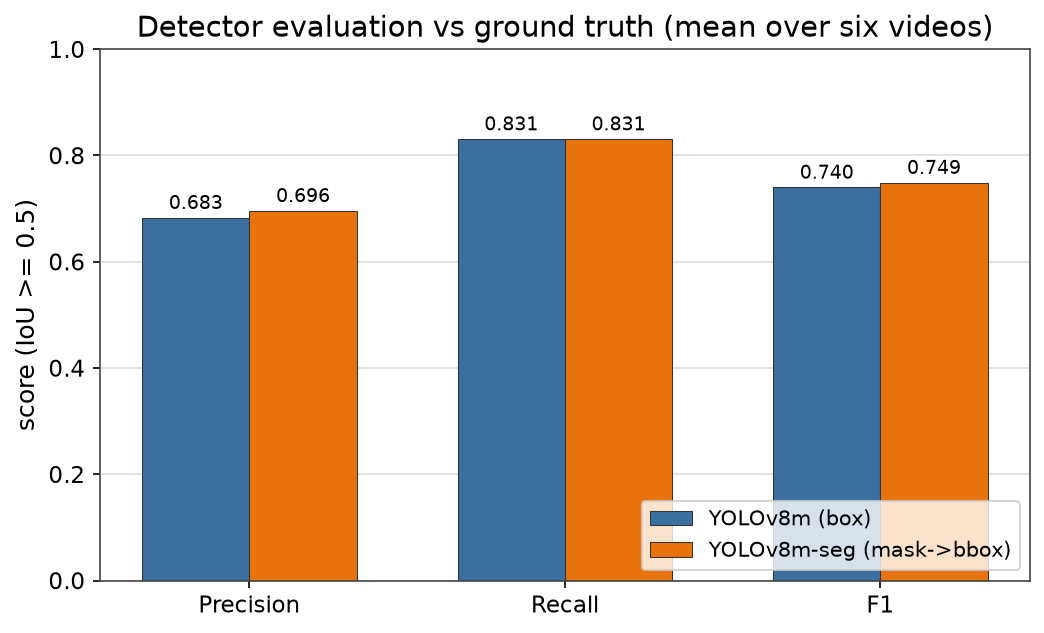
\includegraphics[width=0.7\textwidth]{fig_detector_prf.png}
  \caption{Detector precision, recall and F1 for the box and segmentation YOLOv8m variants.}
  \label{fig:detprf}
\end{figure}

\subsection{Re-Identification Study}
With detection fixed to ground truth, \hota{} reflects association quality. \osnet{} is the strongest
appearance model (mean \hota{} $89.93$), narrowly ahead of the \texttt{timm} backbone ($89.22$),
followed by \osnet{}-AIN ($87.33$) and the smaller \osnet{}-x0.25 ($86.13$); see
Figure~\ref{fig:reidonly}. The high absolute values are expected because ground-truth boxes make
detection near-perfect.

\begin{figure}[H]
  \centering
  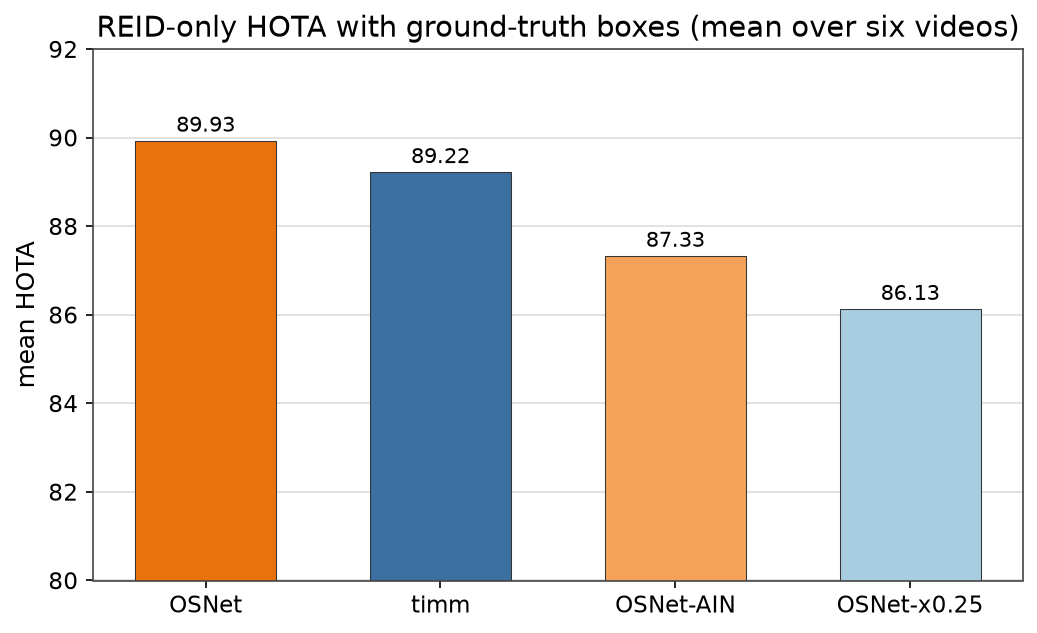
\includegraphics[width=0.65\textwidth]{fig_reid_only.png}
  \caption{Re-identification-only \hota{} with ground-truth boxes (mean over six videos).}
  \label{fig:reidonly}
\end{figure}

\subsection{Full Pipeline}
Table~\ref{tab:fullpipeline} and Figure~\ref{fig:hota} report the live pipeline. The best
configuration, YOLOv8m with \osnet{}, reaches a mean \hota{} of $52.54$ ($+12.37$ over the baseline)
and exceeds the baseline on each of the six videos. The \texttt{timm} configuration reaches $47.70$.

\begin{table}[H]
\centering
\caption{Per-video \hota{}: baseline and the two modern configurations. The YOLOv8m + \osnet{} row
uses the tuned TUD-Campus preset (Section~\ref{sec:tuning}).}
\label{tab:fullpipeline}
\small
\setlength{\tabcolsep}{4.5pt}
\begin{tabular}{lccccccc}
\toprule
\textbf{Configuration} & TUD-Campus & TUD-Stadt. & KITTI-17 & PETS09 & MOT16-09 & MOT16-11 & \textbf{Mean} \\
\midrule
Baseline                 & 39.86 & 36.75 & 43.41 & 44.84 & 36.24 & 39.95 & 40.17 \\
YOLOv8m + timm           & 37.57 & 57.63 & 45.82 & 50.89 & 45.56 & 48.73 & 47.70 \\
\textbf{YOLOv8m + OSNet} & \textbf{46.98} & \textbf{59.62} & \textbf{48.75} & \textbf{60.28} & \textbf{48.57} & \textbf{51.07} & \textbf{52.54} \\
\bottomrule
\end{tabular}
\end{table}

\begin{figure}[H]
  \centering
  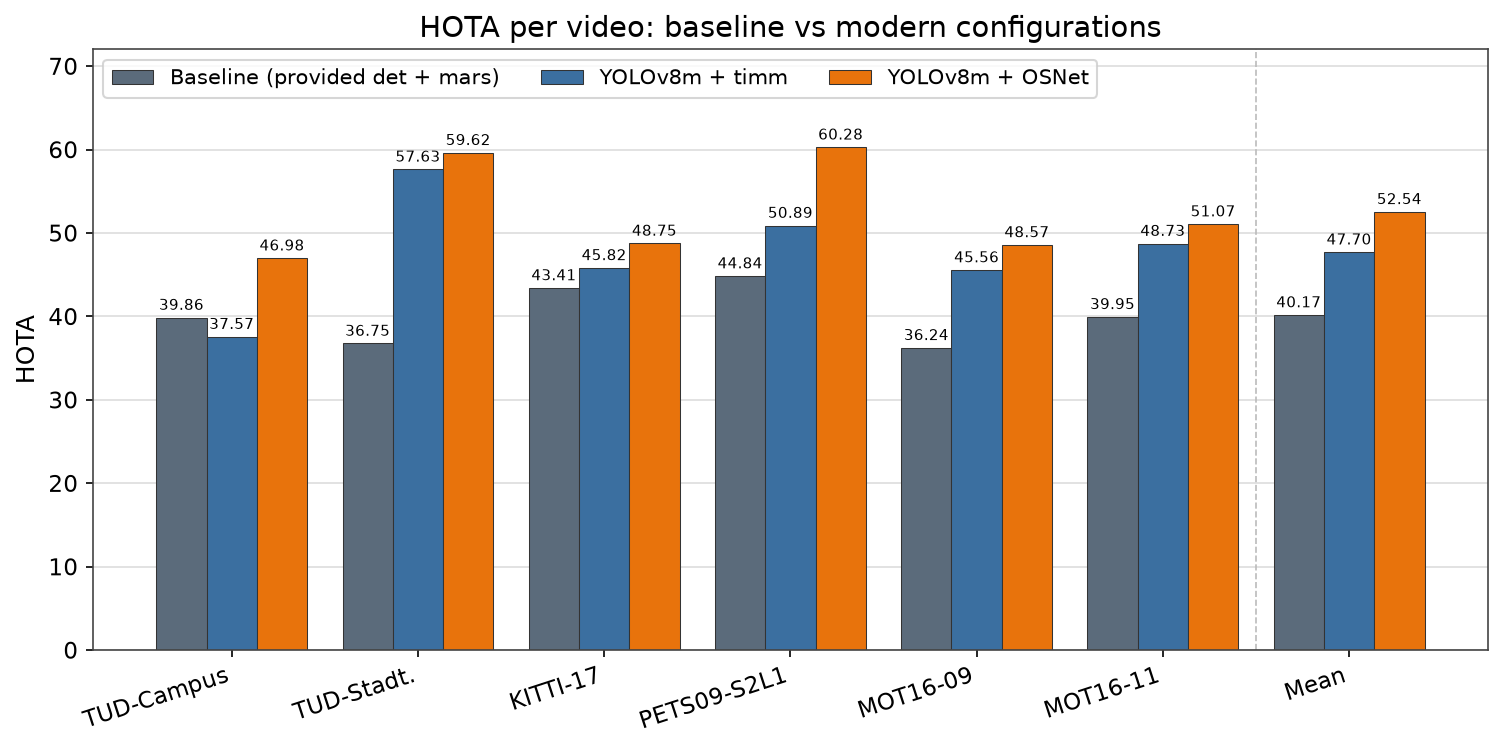
\includegraphics[width=0.95\textwidth]{fig_hota_per_video.png}
  \caption{Per-video \hota{} for the baseline and the two modern configurations.}
  \label{fig:hota}
\end{figure}

\subsection{TUD-Campus Tuning Case Study}
\label{sec:tuning}
TUD-Campus was the only video on which the modern configuration initially trailed the baseline
($39.65$ versus $39.86$). Two sweeps were run with \texttt{eval/tune\_tud\_campus.py}, both expressed
through the TUD-Campus sequence preset (the live runner has no command-line override mechanism).
\begin{itemize}
  \item A recall-direction sweep (increasing \texttt{detector.imgsz} from $960$ to $1280$ and $1536$,
        and lowering the confidence threshold) was not supported by the data: \hota{} fell
        monotonically ($39.65 \rightarrow 35.0 \rightarrow 29.7$). Additional detections reduced the
        score.
  \item A precision-direction sweep was supported. The live pipeline applies no non-maximum
        suppression (\texttt{tracker.nms\_max\_overlap} default $1.0$) and no separate confidence gate
        (\texttt{tracker.min\_confidence} default $0.0$), so the many low-confidence false positives
        on this dense clip are admitted to the tracker and create spurious tracks. Raising
        \texttt{detector.conf} to $0.45$ reduces the false-positive count and raises \hota{} to
        $46.98$ ($+7.1$ over the baseline).
\end{itemize}
Table~\ref{tab:sweep} and Figure~\ref{fig:sweep} report the sweep. The change is confined to the
TUD-Campus preset; the other five sequences are unchanged.

\begin{table}[H]
\centering
\caption{TUD-Campus tuning sweep. Configurations above the baseline ($39.86$) are in the upper rows.}
\label{tab:sweep}
\begin{tabular}{lc@{\hskip 2cm}lc}
\toprule
\textbf{Configuration} & \textbf{HOTA} & \textbf{Configuration} & \textbf{HOTA} \\
\midrule
conf 0.45 (selected)   & \textbf{46.98} & min\_height 20          & 39.85 \\
conf 0.35              & 44.61          & control (conf 0.25)     & 39.65 \\
nms 0.7 + conf 0.35    & 42.49          & nms 0.7 alone           & 38.40 \\
min\_confidence 0.30   & 42.22          & imgsz 1280              & 35.03 \\
nms\_max\_overlap 0.5  & 41.96          & imgsz 1536              & 29.75 \\
nms 0.7 + minconf + h15 & 40.39         &                         &       \\
\bottomrule
\end{tabular}
\end{table}

\begin{figure}[H]
  \centering
  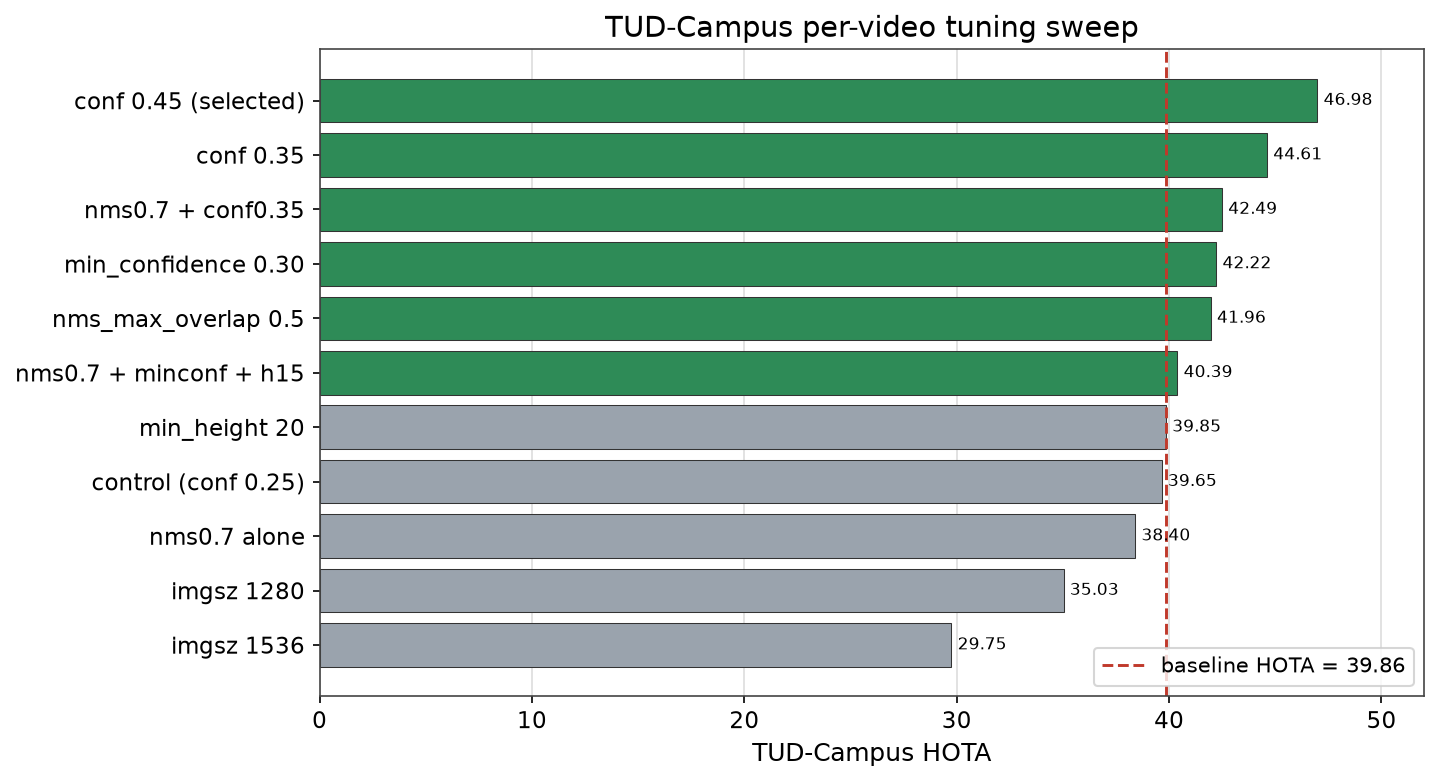
\includegraphics[width=0.8\textwidth]{fig_tuning_sweep.png}
  \caption{TUD-Campus tuning sweep. The dashed line is the baseline \hota{}.}
  \label{fig:sweep}
\end{figure}

\subsection{Metric Decomposition}
Table~\ref{tab:decomp} and Figure~\ref{fig:decomp} decompose the improvement on the combined MOT16
split for YOLOv8m + timm. Most of the gain is on the detection term (DetA $+12.30$); the association
term also improves (AssA $+6.25$). MOTA changes little, which is consistent with the fact that MOTA
is dominated by detection recall.

\begin{table}[H]
\centering
\caption{Metric decomposition on the combined MOT16 split (YOLOv8m + timm vs baseline).}
\label{tab:decomp}
\begin{tabular}{lccccc}
\toprule
\textbf{Configuration} & HOTA & MOTA & IDF1 & DetA & AssA \\
\midrule
Baseline (provided det + mars) & 38.65 & 46.34 & 50.65 & 37.85 & 39.52 \\
Modern (YOLOv8m + timm)        & 47.68 & 46.75 & 52.18 & 50.15 & 45.77 \\
\midrule
Difference                     & $+9.03$ & $+0.41$ & $+1.53$ & $+12.30$ & $+6.25$ \\
\bottomrule
\end{tabular}
\end{table}

\begin{figure}[H]
  \centering
  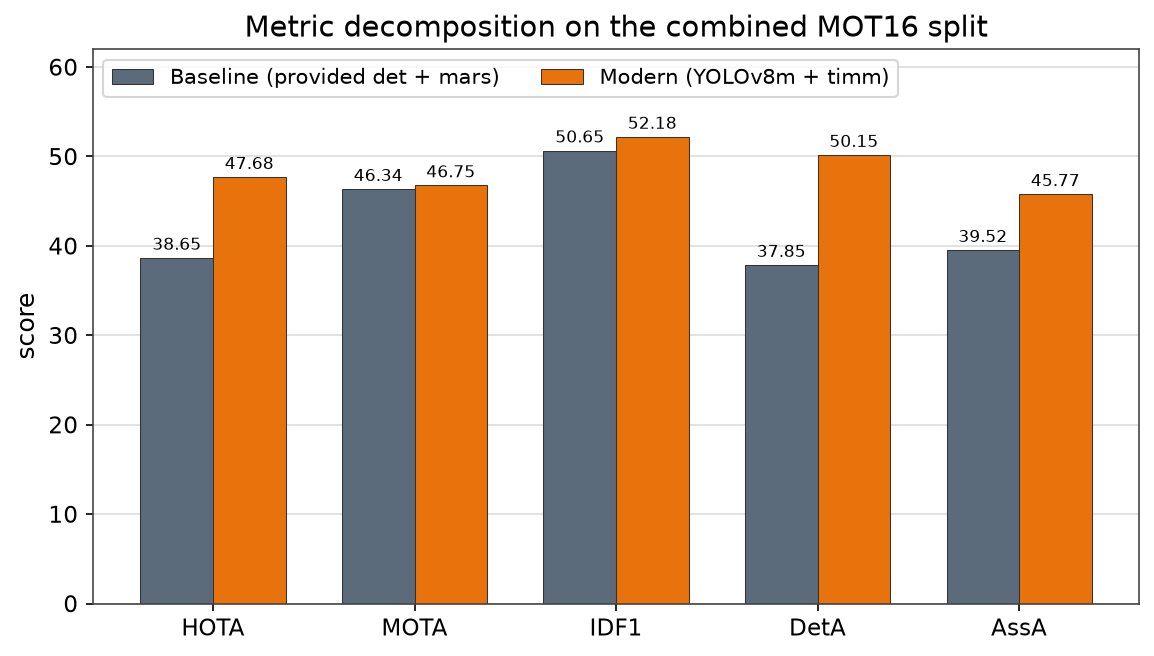
\includegraphics[width=0.8\textwidth]{fig_metric_decomposition.png}
  \caption{Metric decomposition on the combined MOT16 split.}
  \label{fig:decomp}
\end{figure}

\subsection{Segmentation}
The YOLOv8 segmentation detector produces a person mask and converts it to a tight bounding box. It
is marginally better than the box detector on detection F1 ($0.768$ vs $0.765$) and on mean
\hota{} ($52.76$ vs $52.54$), but the mask head is substantially slower: on MOT16-09 the segmentation
pipeline runs at $3.92$~FPS, below the $5$~FPS real-time threshold, against $9.87$~FPS for the box
pipeline. Segmentation stays real-time on the lighter 2D~MOT~2015 clips ($\sim$10--14~FPS) but not on
the heavier MOT16 sequences. The marginal accuracy gain therefore does not justify the loss of
real-time throughput, so the box detector is the default and segmentation is a switchable option
(Figure~\ref{fig:seg}).

\begin{figure}[H]
  \centering
  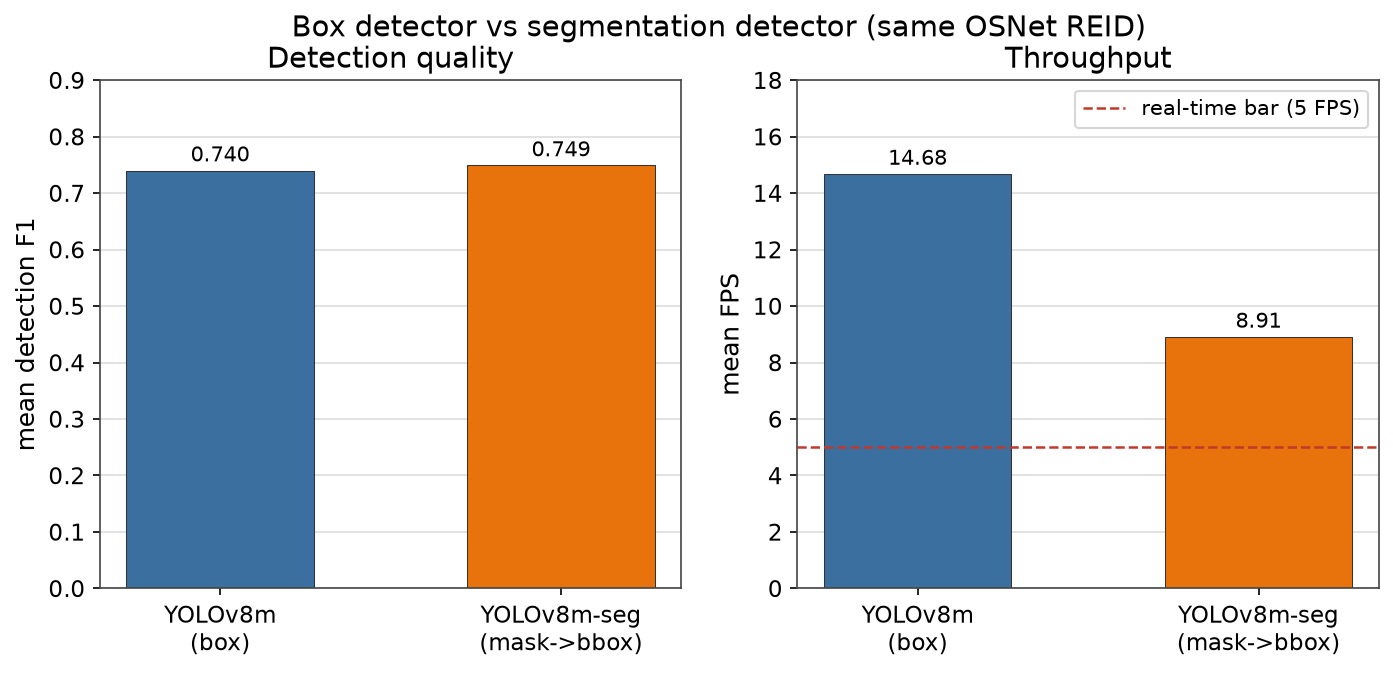
\includegraphics[width=0.85\textwidth]{fig_segmentation.png}
  \caption{Box detector versus segmentation detector with the same \osnet{} re-identification model.}
  \label{fig:seg}
\end{figure}

\subsection{Standalone Body-REID}
The standalone body-\reid{} component was evaluated as a clustering problem on the $21{,}105$
ground-truth crops ($140$ true identities) using \osnet{} descriptors. In the embedding mode
(agglomerative clustering at the default threshold) the predicted number of identities is too high
($420$ vs $140$, Fowlkes-Mallows index $0.630$); in the assignment mode (a headless replay of the
identity database) it is too low ($30$ vs $140$, Fowlkes-Mallows index $0.242$). The two modes
bracket the true count, which indicates that the default thresholds should be tuned toward
$n_{\text{pred}} \approx n_{\text{true}}$; the sweep utility \texttt{bodyreid/eval/sweep.py} exists
for this purpose. Figure~\ref{fig:bodyreid} shows the predicted counts against the true count.

\begin{table}[H]
\centering
\caption{Standalone body-\reid{} clustering metrics (\osnet{} descriptors, 21,105 crops, 140 true identities).}
\label{tab:bodyreid}
\begin{tabular}{lcccc}
\toprule
\textbf{Mode} & \textbf{Fowlkes-Mallows} & \textbf{Silhouette} & \textbf{Calinski-Harabasz} & $n_{\text{pred}}/n_{\text{true}}$ \\
\midrule
Embedding (agglomerative) & 0.630 & 0.371 & 98.3 & 420 / 140 \\
Assignment (DB replay)    & 0.242 & --    & --   & 30 / 140 \\
\bottomrule
\end{tabular}
\end{table}

\begin{figure}[H]
  \centering
  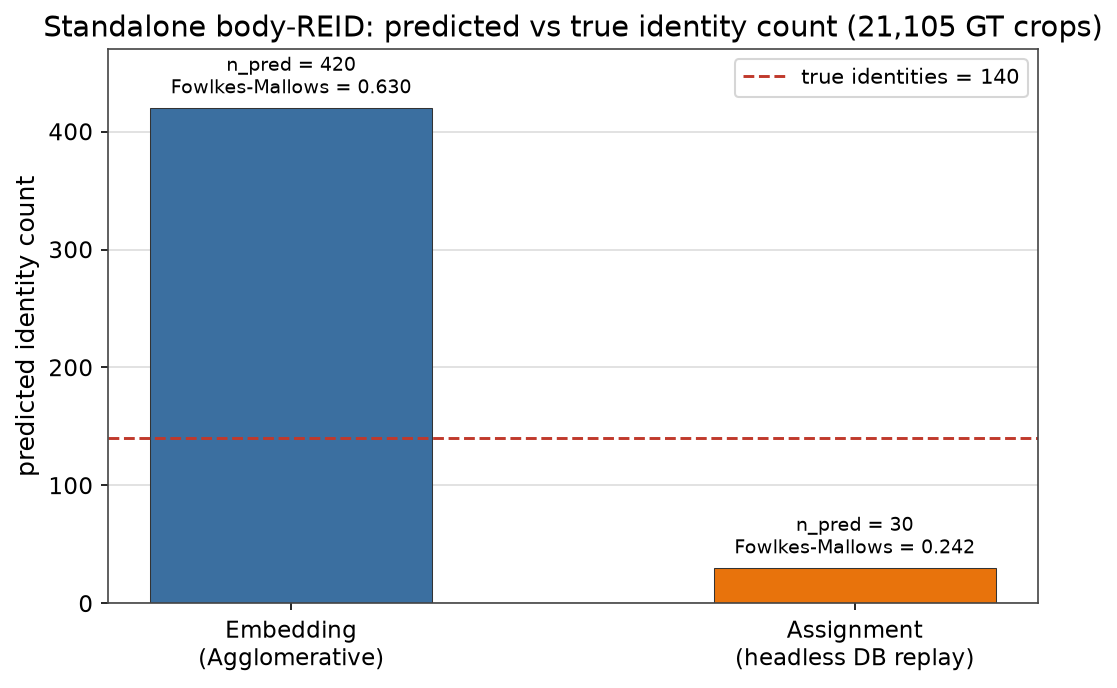
\includegraphics[width=0.65\textwidth]{fig_bodyreid_cluster.png}
  \caption{Standalone body-\reid{}: predicted identity count in each mode against the true count.}
  \label{fig:bodyreid}
\end{figure}

\subsection{Real-Time Performance}
On MOT16-09, the YOLOv8m + \osnet{} configuration runs at $9.87$~FPS overall, above the $5$~FPS
threshold. Figure~\ref{fig:latency} shows the per-frame time by stage: the detector and
re-identification stages dominate, while the tracking core is comparatively cheap.

\begin{figure}[H]
  \centering
  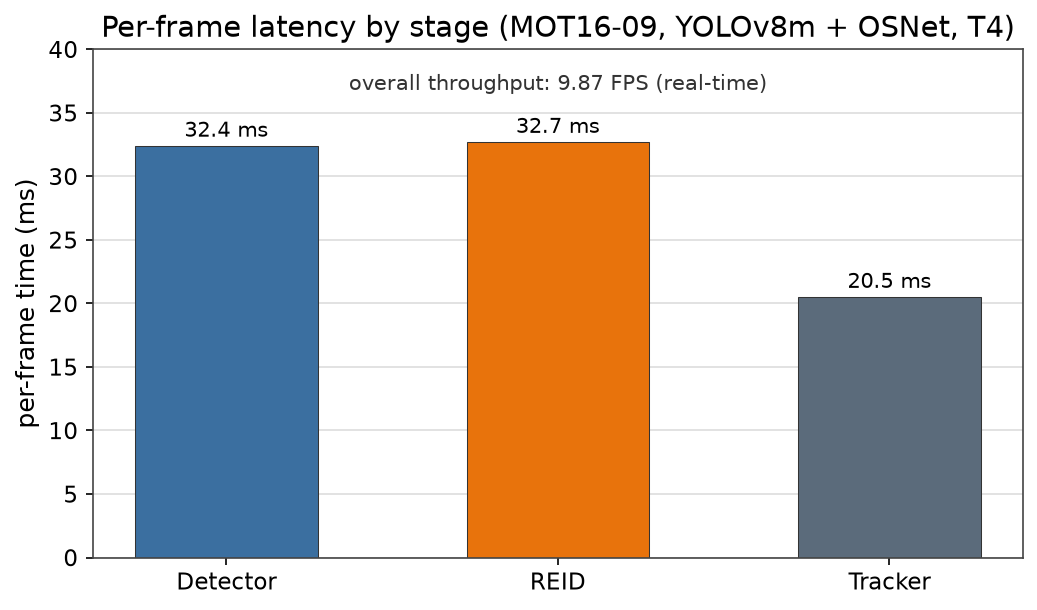
\includegraphics[width=0.7\textwidth]{fig_stage_latency.png}
  \caption{Per-frame latency by stage (MOT16-09, YOLOv8m + \osnet{}, Tesla T4).}
  \label{fig:latency}
\end{figure}

% ----------------------------------------------------------------------------
%  5. METHODS AND TECHNOLOGIES
% ----------------------------------------------------------------------------
\section{Methods and Technologies}
\label{sec:methods}

\subsection{Detector and REID Adapters}
Each detector adapter normalizes its output to person-only boxes in \texttt{tlwh} format with a
confidence score; the COCO person class index, which differs between frameworks, is handled in the
base class rather than hard-coded. Each \reid{} adapter maps cropped images to L2-normalized
embeddings; the cosine metric in the tracking core is dimension-agnostic, so different embedding
sizes are interchangeable.

\subsection{Standalone Body-REID Algorithm}
\label{sec:bodyreid-method}
The standalone identity component maintains a persistent identity database that is decoupled from the
tracker's ephemeral track identities. Each identity keeps a running centroid and a capped gallery of
recent descriptors. A new detection is matched by cosine distance with two thresholds: a match
threshold below which the detection is assigned and enrolled, a higher threshold above which a new
identity may be created only at track birth, and an intermediate band in which the detection is
assigned but not enrolled. A per-track history is resolved over a time window by distance-weighted
majority vote with hysteresis, and a cross-track conflict rule prevents two simultaneously active
tracks from sharing one identity. The component is evaluated on its own terms as a clustering problem
(Section~\ref{sec:results}); it reads tracker output through a per-frame hook and does not modify the
tracking core.

\subsection{Technology Stack}
\begin{table}[H]
\centering
\caption{Main software components.}
\label{tab:stack}
\begin{tabular}{ll}
\toprule
\textbf{Component} & \textbf{Role} \\
\midrule
PyTorch, Ultralytics & detector inference (YOLOv8m, YOLOv8-seg) \\
BoxMOT, torchreid, timm & re-identification backends \\
TrackEval & HOTA / MOTA / IDF1 scoring \\
scikit-learn & precision/recall/F1 and clustering metrics \\
NumPy, OpenCV & array and image operations \\
Google Colab Pro (Tesla T4) & compute environment \\
\bottomrule
\end{tabular}
\end{table}

% ----------------------------------------------------------------------------
%  6. DIFFICULTIES
% ----------------------------------------------------------------------------
\section{Deviations and Difficulties}
\label{sec:difficulties}

This section records the problems encountered, including the cases that did not work. Most were
environment issues on the bleeding-edge Colab runtime (Python~3.12, NumPy~2.x) rather than algorithm
problems.

\begin{table}[H]
\centering
\caption{Difficulties encountered and how they were handled.}
\label{tab:difficulties}
\begin{tabular}{p{0.42\textwidth} p{0.5\textwidth}}
\toprule
\textbf{Problem} & \textbf{Resolution} \\
\midrule
torchreid does not build under NumPy~2.x (metadata-generation failure). & The torchreid path to \osnet{} was blocked; \osnet{} was obtained through BoxMOT instead. \\
BoxMOT initially failed to build and is an optional dependency. & It is installed in a guarded step (\texttt{pip install boxmot \textbar\textbar\ echo ...}) and excluded from the hard requirements set, so its failure cannot abort the core install. It built successfully in the final run, which unblocked \osnet{}. \\
A dependency-light \reid{} was needed as a fallback. & A \texttt{timm} ImageNet backbone (not re-identification-trained) is used; it installs without a native build and still exceeds the baseline. \\
TrackEval uses removed NumPy aliases (\texttt{np.float}, \texttt{np.int}, \texttt{np.bool}). & The TrackEval source is patched in place at run time before scoring. \\
2D~MOT~2015 ground truth is 10-column (columns 7--9 are world coordinates), while MOT16 is 9-column (class and visibility). & The loader reads class and visibility only when there are exactly nine columns; a regression test fixes both formats. The earlier code silently dropped the four 2D~MOT~2015 sequences. \\
The official MOT-Challenge host was unreachable from Colab. & A mirror that preserves the MOT-Challenge directory layout is used; the official URLs remain configurable. \\
The notebook used IPython shell-variable substitution across cells, which expanded to empty values. & A configuration cell exports the values to the shell environment, so the \texttt{!} cells receive real environment variables. \\
\bottomrule
\end{tabular}
\end{table}

% ----------------------------------------------------------------------------
%  7. CONCLUSION
% ----------------------------------------------------------------------------
\section{Conclusion}
\label{sec:conclusion}

The modernized DeepSORT replaces the fixed detector and appearance encoder of the reference
implementation with selectable modern models behind two adapter interfaces, while keeping the SORT
core unchanged. On the six MOT-Challenge evaluation videos, the best configuration (YOLOv8m with an
\osnet{} re-identification model) reaches a mean \hota{} of $52.54$ versus $40.17$ for the unmodified
baseline ($+12.37$), exceeds the baseline on every video, and runs at $9.87$~FPS on a Tesla~T4. The
improvement is driven mainly by detection quality (DetA $+12.30$) and, to a smaller degree, by
association (AssA $+6.25$). A per-video tuning study on TUD-Campus showed that the binding constraint
there was an excess of low-confidence detections rather than insufficient recall, and that raising the
detector confidence threshold closed the gap. The standalone body-\reid{} component is implemented and
evaluated as a clustering problem; its default thresholds bracket the true identity count and are a
clear target for the existing parameter sweep.

\subsection{Future Directions}
The threshold sweep for the standalone body-\reid{} component, the measurement of its effect on the
end-to-end tracking metrics, and the installation of the NanoDet and RTMDet detectors on a compatible
runtime are the natural next steps. A torchreid build compatible with NumPy~2.x would allow the
remaining \osnet{} variants and a ResNet-50 re-identification model to be measured in the same study.

% ----------------------------------------------------------------------------
%  BIBLIOGRAPHY
% ----------------------------------------------------------------------------
\newpage
\begin{thebibliography}{99}

\bibitem{bewley2016sort}
A.~Bewley, Z.~Ge, L.~Ott, F.~Ramos, and B.~Upcroft.
\newblock {Simple Online and Realtime Tracking}.
\newblock In \emph{IEEE International Conference on Image Processing (ICIP)}, pages 3464--3468, 2016.
\newblock \href{https://arxiv.org/abs/1602.00763}{arXiv:1602.00763}.

\bibitem{wojke2017deepsort}
N.~Wojke, A.~Bewley, and D.~Paulus.
\newblock {Simple Online and Realtime Tracking with a Deep Association Metric}.
\newblock In \emph{IEEE International Conference on Image Processing (ICIP)}, pages 3645--3649, 2017.
\newblock \href{https://arxiv.org/abs/1703.07402}{arXiv:1703.07402}.

\bibitem{wojke2018cosine}
N.~Wojke and A.~Bewley.
\newblock {Deep Cosine Metric Learning for Person Re-Identification}.
\newblock In \emph{IEEE Winter Conference on Applications of Computer Vision (WACV)}, pages 748--756, 2018.
\newblock \href{https://arxiv.org/abs/1812.00442}{arXiv:1812.00442}.

\bibitem{luiten2021hota}
J.~Luiten, A.~Osep, P.~Dendorfer, P.~Torr, A.~Geiger, L.~Leal-Taixe, and B.~Leibe.
\newblock {HOTA: A Higher Order Metric for Evaluating Multi-Object Tracking}.
\newblock \emph{International Journal of Computer Vision}, 129(2):548--578, 2021.
\newblock \href{https://arxiv.org/abs/2009.07736}{arXiv:2009.07736}.

\bibitem{trackeval}
J.~Luiten and A.~Hoffhues.
\newblock {TrackEval}.
\newblock \url{https://github.com/JonathonLuiten/TrackEval}, 2020. Accessed: 2026-06-19.

\bibitem{leal2015motchallenge}
L.~Leal-Taixe, A.~Milan, I.~Reid, S.~Roth, and K.~Schindler.
\newblock {MOTChallenge 2015: Towards a Benchmark for Multi-Target Tracking}.
\newblock \href{https://arxiv.org/abs/1504.01942}{arXiv:1504.01942}, 2015.

\bibitem{milan2016mot16}
A.~Milan, L.~Leal-Taixe, I.~Reid, S.~Roth, and K.~Schindler.
\newblock {MOT16: A Benchmark for Multi-Object Tracking}.
\newblock \href{https://arxiv.org/abs/1603.00831}{arXiv:1603.00831}, 2016.

\bibitem{jocher2023yolov8}
G.~Jocher, A.~Chaurasia, and J.~Qiu.
\newblock {Ultralytics YOLOv8}.
\newblock \url{https://github.com/ultralytics/ultralytics}, 2023. Accessed: 2026-06-19.

\bibitem{zhou2019osnet}
K.~Zhou, Y.~Yang, A.~Cavallaro, and T.~Xiang.
\newblock {Omni-Scale Feature Learning for Person Re-Identification}.
\newblock In \emph{IEEE/CVF International Conference on Computer Vision (ICCV)}, pages 3702--3712, 2019.
\newblock \href{https://arxiv.org/abs/1905.00953}{arXiv:1905.00953}.

\bibitem{zhou2021torchreid}
K.~Zhou and T.~Xiang.
\newblock {Torchreid: A Library for Deep Learning Person Re-Identification in PyTorch}.
\newblock \href{https://arxiv.org/abs/1910.10093}{arXiv:1910.10093}, 2019.

\bibitem{brostrom2023boxmot}
M.~Brostrom.
\newblock {BoxMOT: Pluggable SOTA Tracking Modules for Detection and Segmentation Models}.
\newblock \url{https://github.com/mikel-brostrom/boxmot}, 2023. Accessed: 2026-06-19.

\bibitem{wightman2019timm}
R.~Wightman.
\newblock {PyTorch Image Models (timm)}.
\newblock \url{https://github.com/huggingface/pytorch-image-models}, 2019. Accessed: 2026-06-19.

\bibitem{lyu2022rtmdet}
C.~Lyu, W.~Zhang, H.~Huang, Y.~Zhou, Y.~Wang, Y.~Liu, S.~Zhang, and K.~Chen.
\newblock {RTMDet: An Empirical Study of Designing Real-Time Object Detectors}.
\newblock \href{https://arxiv.org/abs/2212.07784}{arXiv:2212.07784}, 2022.

\bibitem{mmdetection}
K.~Chen, J.~Wang, J.~Pang, et~al.
\newblock {MMDetection: Open MMLab Detection Toolbox and Benchmark}.
\newblock \href{https://arxiv.org/abs/1906.07155}{arXiv:1906.07155}, 2019.

\bibitem{rangilyu2021nanodet}
RangiLyu.
\newblock {NanoDet-Plus: Super Fast and High Accuracy Lightweight Anchor-Free Object Detection Model}.
\newblock \url{https://github.com/RangiLyu/nanodet}, 2021. Accessed: 2026-06-19.

\end{thebibliography}

\end{document}
